\ifx\type\undefined
  \documentclass[10pt, t]{beamer}
  \setbeamertemplate{footline}[page number]
\else
  \documentclass[10pt]{article}
  \usepackage[margin=1in]{geometry}
\fi

\usepackage{amsmath}
\usepackage{amssymb}
\usepackage{amsthm}
\usepackage{bbm}
\usepackage{cancel}
\usepackage{listings}
\usepackage{mathrsfs}
\usepackage{multirow}
\usepackage{soul}
\usepackage{stmaryrd}
\usepackage{tikz}
\usepackage{tikz-cd}
\usepackage{wrapfig}

\newtheorem*{algorithm}{Algorithm}
\newtheorem*{assumptions}{Assumptions}
\newtheorem*{conjecture}{Conjecture}
\newtheorem*{consequences}{Consequences}
\newtheorem*{exercise}{Exercise}
\newtheorem*{formalisation}{Formalisation}
\newtheorem*{proposition}{Proposition}
\newtheorem*{question}{Question}
\newtheorem*{remark}{Remark}

\ifx\type\undefined\else
  \newtheorem*{definition}{Definition}
  \newtheorem*{example}{Example}
  \newtheorem*{lemma}{Lemma}
  \newtheorem*{theorem}{Theorem}
\fi

\definecolor{keywordcolor}{rgb}{0.7, 0.1, 0.1}
\definecolor{tacticcolor}{rgb}{0.0, 0.1, 0.6}
\definecolor{commentcolor}{rgb}{0.4, 0.4, 0.4}
\definecolor{symbolcolor}{rgb}{0.0, 0.1, 0.6}
\definecolor{sortcolor}{rgb}{0.1, 0.5, 0.1}
\definecolor{attributecolor}{rgb}{0.7, 0.1, 0.1}
\def\lstlanguagefiles{lstlean.tex}
\lstset{language=lean}

\newcommand\A{\mathbb{A}}
\newcommand\C{\mathbb{C}}
\newcommand\F{\mathbb{F}}
\newcommand\G{\mathbb{G}}
\renewcommand\H{\mathbb{H}}
\newcommand\I{\mathbb{I}}
\newcommand\N{\mathbb{N}}
\renewcommand\P{\mathbb{P}}
\newcommand\Q{\mathbb{Q}}
\newcommand\R{\mathbb{R}}
\newcommand\Z{\mathbb{Z}}

\renewcommand\AA{\mathcal{A}}
\newcommand\BB{\mathcal{B}}
\newcommand\CC{\mathcal{C}}
\newcommand\DD{\mathcal{D}}
\newcommand\EE{\mathcal{E}}
\newcommand\FF{\mathcal{F}}
\newcommand\GG{\mathcal{G}}
\newcommand\HH{\mathcal{H}}
\newcommand\II{\mathcal{I}}
\newcommand\LL{\mathcal{L}}
\newcommand\MM{\mathcal{M}}
\newcommand\NN{\mathcal{N}}
\newcommand\OO{\mathcal{O}}
\newcommand\PP{\mathcal{P}}
\newcommand\RR{\mathcal{R}}
\renewcommand\SS{\mathcal{S}}
\newcommand\TT{\mathcal{T}}
\newcommand\XX{\mathcal{X}}

\renewcommand\aa{\mathfrak{a}}
\newcommand\cc{\mathfrak{c}}
\newcommand\dd{\mathfrak{d}}
\newcommand\ff{\mathfrak{f}}
\renewcommand\gg{\mathfrak{g}}
\newcommand\mm{\mathfrak{m}}
\newcommand\pp{\mathfrak{p}}
\newcommand\qq{\mathfrak{q}}
\renewcommand\ss{\mathfrak{s}}

\newcommand\LLL{\mathscr{L}}

\newcommand\ab{\mathrm{ab}}
\newcommand\Ab{\mathbf{Ab}}
\newcommand\Alg{\mathbf{Alg}}
\newcommand\Aff{\mathbf{Aff}}
\newcommand\Aut{\operatorname{Aut}}
\newcommand\Az{\mathrm{Az}}
\newcommand\Br{\operatorname{Br}}
\newcommand\BSD{\operatorname{BSD}}
\newcommand\ch{\operatorname{char}}
\newcommand\Cl{\operatorname{Cl}}
\newcommand\coker{\operatorname{coker}}
\newcommand\cris{\mathrm{cris}}
\renewcommand\d{\mathrm{d}}
\newcommand\Div{\operatorname{Div}}
\newcommand\dR{\mathrm{dR}}
\newcommand\EN{\operatorname{EN}}
\newcommand\End{\operatorname{End}}
\newcommand\ES{\operatorname{ES}}
\newcommand\et{\mathrm{\acute{e}t}}
\newcommand\Et{\mathbf{\acute{E}t}}
\newcommand\Ext{\operatorname{Ext}}
\newcommand\Fr{\operatorname{Fr}}
\newcommand\Frac{\operatorname{Frac}}
\newcommand\Gal{\operatorname{Gal}}
\newcommand\GL{\operatorname{GL}}
\newcommand\Gr{\mathrm{Gr}}
\newcommand\Hom{\operatorname{Hom}}
\newcommand\HT{\mathrm{HT}}
\newcommand\id{\operatorname{id}}
\newcommand\im{\operatorname{im}}
\newcommand\Ind{\operatorname{Ind}}
\renewcommand\inf{\operatorname{inf}}
\newcommand\inv{\operatorname{inv}}
\newcommand\Irr{\operatorname{Irr}}
\newcommand\Jac{\operatorname{Jac}}
\newcommand\lcm{\operatorname{lcm}}
\newcommand\Mat{\operatorname{Mat}}
\newcommand\Mod{\mathbf{Mod}}
\newcommand\Nm{\operatorname{Nm}}
\newcommand\nr{\mathrm{nr}}
\newcommand\NS{\operatorname{NS}}
\newcommand\Ob{\operatorname{Ob}}
\newcommand\ord{\operatorname{ord}}
\newcommand\op{\mathrm{op}}
\newcommand\PGL{\operatorname{PGL}}
\newcommand\Pic{\operatorname{Pic}}
\newcommand\Prob{\operatorname{Prob}}
\newcommand\Proj{\operatorname{Proj}}
\newcommand\PSh{\mathbf{PSh}}
\newcommand\Reg{\operatorname{Reg}}
\newcommand\res{\operatorname{res}}
\newcommand\rk{\operatorname{rk}}
\newcommand\Sch{\mathbf{Sch}}
\newcommand\Sel{\operatorname{Sel}}
\newcommand\Set{\mathbf{Set}}
\newcommand\sgn{\operatorname{sgn}}
\newcommand\Sh{\mathbf{Sh}}
\newcommand\SL{\operatorname{SL}}
\newcommand\Spec{\operatorname{Spec}}
\newcommand\supp{\operatorname{supp}}
\newcommand\Tam{\operatorname{Tam}}
\newcommand\Top{\mathbf{Top}}
\newcommand\tor{\operatorname{tor}}
\newcommand\tr{\operatorname{tr}}
\newcommand\tra{\operatorname{tra}}
\newcommand\WC{\operatorname{WC}}

\DeclareFontFamily{U}{wncyr}{}
\DeclareFontShape{U}{wncyr}{m}{n}{<->wncyr10}{}
\DeclareSymbolFont{cyr}{U}{wncyr}{m}{n}
\DeclareMathSymbol{\Sha}{\mathord}{cyr}{"58}

\newcommand{\function}[5][]{
  \if &#1&
    \begin{array}{rcl}
      #2 & \longrightarrow & #3 \\
      #4 & \longmapsto     & #5
    \end{array}
  \else
    \begin{array}{rcrcl}
      #1 & : & #2 & \longrightarrow & #3 \\
         &   & #4 & \longmapsto     & #5
    \end{array}
  \fi
}

\newcommand{\functions}[7][]{
  \if &#1&
    \begin{array}{rcl}
      #2 & \longrightarrow & #3 \\
      #4 & \longmapsto     & #5 \\
      #6 & \longmapsto     & #7 \\
    \end{array}
  \else
    \begin{array}{rcrcl}
      #1 & : & #2 & \longrightarrow & #3 \\
         &   & #4 & \longmapsto     & #5 \\
         &   & #6 & \longmapsto     & #7
    \end{array}
  \fi
}
\title{Arithmetic statistics for elliptic curves}
\subtitle{Master's thesis presentation}
\author{David Kurniadi Angdinata}
\institute{Imperial College London}
\date{Monday, 22 June 2020}

\begin{document}

\frame\maketitle

\begin{frame}{Some motivation}

What are elliptic curves?
\begin{itemize}
\item Solutions to $ y^2 = x^3 + ax + b $ for rational numbers $ a $ and $ b $.
\end{itemize}

\begin{center}
\includegraphics[width=0.4\textwidth]{img/ellipticcurve.png}
\end{center}

What are they used for?
\begin{itemize}
\item Number theory.
\item Cryptography.
\end{itemize}

\end{frame}

\begin{frame}{Some motivation}

What do we know?
\begin{itemize}
\item It is a group.
\item It has a rank.
\end{itemize}
What do we not know?
\begin{itemize}
\item What is the average rank?
\begin{itemize}
\item Probably $ \tfrac{1}{2} $.
\end{itemize}
\item How large can the rank be?
\begin{itemize}
\item At least $ 28 $.
\end{itemize}
\item Is the rank bounded?
\begin{itemize}
\item Maybe?
\end{itemize}
\end{itemize}
What can we do?
\begin{itemize}
\item Study Selmer groups and Tate--Shafarevich groups.
\item Neither are easy to study.
\item Study models for them instead.
\end{itemize}

\end{frame}

\begin{frame}[c]{Framework and overview}

\begin{center}
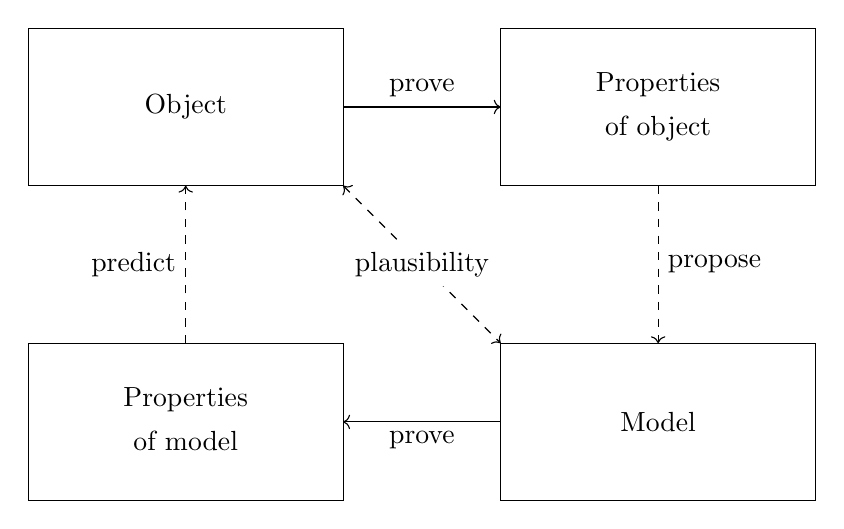
\begin{tikzpicture}
\draw (-1, 1) rectangle node{Object} (-5, 3);
\draw [->] (-1, 2) to node[above]{prove} (1, 2);
\draw (1, 1) rectangle node[above]{Properties} node[below]{of object} (5, 3);
\draw [->, dashed] (3, 1) to node[right]{propose} (3, -1);
\draw (1, -1) rectangle node{Model} (5, -3);
\draw [->] (1, -2) to node[below]{prove} (-1, -2);
\draw (-1, -1) rectangle node[above]{Properties} node[below]{of model} (-5, -3);
\draw [->, dashed] (-3, -1) to node[left]{predict} (-3, 1);
\draw [<->, dashed] (-1, 1) to node[fill=white]{plausibility} (1, -1);
\end{tikzpicture}
\end{center}

\end{frame}

\begin{frame}[c]{Framework and overview}

\begin{center}
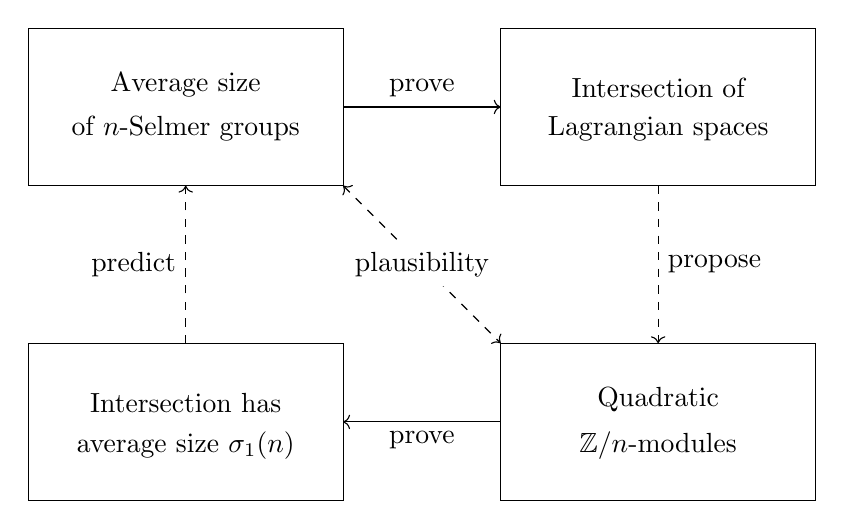
\begin{tikzpicture}
\draw (-1, 1) rectangle node[above]{Average size} node[below]{of $ n $-Selmer groups} (-5, 3);
\draw [->] (-1, 2) to node[above]{prove} (1, 2);
\draw (1, 1) rectangle node[above]{Intersection of} node[below]{Lagrangian spaces} (5, 3);
\draw [->, dashed] (3, 1) to node[right]{propose} (3, -1);
\draw (1, -1) rectangle node[above]{Quadratic} node[below]{$ \Z / n $-modules} (5, -3);
\draw [->] (1, -2) to node[below]{prove} (-1, -2);
\draw (-1, -1) rectangle node[above]{Intersection has} node[below]{average size $ \sigma_1(n) $} (-5, -3);
\draw [->, dashed] (-3, -1) to node[left]{predict} (-3, 1);
\draw [<->, dashed] (-1, 1) to node[fill=white]{plausibility} (1, -1);
\end{tikzpicture}
\end{center}

\end{frame}

\begin{frame}[c]{Framework and overview}

``Modelling the Selmer group, the Tate--Shafarevich group, and the Mordell--Weil rank of elliptic curves over number fields''

\bigskip

\begin{theorem}[1) (idea]
The $ n $-Selmer group is usually the intersection of two Lagrangian spaces.
\end{theorem}

\begin{theorem}[2) (idea]
The intersection of two Lagrangian spaces should have average size $ \sigma_1(n) $.
\end{theorem}

\bigskip ``All but finitely many rational elliptic curves have rank at most $ 21 $''

\end{frame}

\begin{frame}{Preliminary background}

Let $ E $ be an \emph{elliptic curve} defined over a \emph{number field} $ K $.
\begin{itemize}
\item $ K $ is a finite extension of $ \Q $ with a fixed algebraic closure $ \overline{K} $.
\item $ E = E(\overline{K}) $ is a smooth projective plane curve of genus one with a distinguished point $ \OO \in E(K) $.
\item $ \Gal(\overline{K} / K) $ acts on $ E $ with invariants $ E(K) $.
\end{itemize}

\bigskip

\begin{theorem}[Mordell--Weil]
$ E(K) $ is a finitely generated abelian group.
\end{theorem}

\bigskip There is an isomorphism
$$ E(K) \cong \tor(E / K) \times \Z^{\rk(E / K)}. $$
The \textbf{Mordell--Weil rank} is $ \rk(E / K) $.

\end{frame}

\begin{frame}{Preliminary background}

Let $ E $ be an elliptic curve defined over a number field $ K $.

\bigskip Multiplying by $ n \in \N^+ $,
$$ 0 \to E[n] \to E \xrightarrow{[n]} E \to 0. $$
Applying $ \Gal(\overline{K} / K) $ cohomology,
$$
\begin{tikzcd}[ampersand replacement=\&, column sep=tiny]
0 \arrow{r} \& E(K)[n] \arrow{r} \& E(K) \arrow{r} \& E(K) \arrow[in=180, out=0]{dll}[swap]{\delta} \& \\
\& H^1(K, E[n]) \arrow{r} \& H^1(K, E) \arrow{r} \& H^1(K, E) \arrow{r} \& \dots.
\end{tikzcd}
$$
Truncating at $ H^1(K, E[n]) $,
$$
\begin{tikzcd}[ampersand replacement=\&]
0 \longrightarrow E(K) / n \arrow{r} \& H^1(K, E[n]) \arrow{r} \& H^1(K, E)[n] \longrightarrow 0.
\end{tikzcd}
$$

\end{frame}

\begin{frame}{Preliminary background}

Let $ E $ be an elliptic curve defined over a number field $ K $.

\bigskip There is a short exact sequence
$$ 0 \to E(K) / n \to H^1(K, E[n]) \to H^1(K, E)[n] \to 0. $$
Let $ K_v $ be a \emph{completion} of $ K $ with respect to a norm $ |\cdot|_v $. Similarly,
$$ 0 \to \prod_v E(K_v) / n \to \prod_v H^1(K_v, E[n]) \to \prod_v H^1(K_v, E)[n] \to 0. $$
There is a row-exact commutative diagram
$$
\begin{tikzcd}[ampersand replacement=\&, column sep=tiny]
0 \arrow{r} \& E(K) / n \arrow{r} \arrow{d} \& H^1(K, E[n]) \arrow{r} \arrow{d}[swap]{\lambda} \arrow[dashed]{dr}{\sigma} \& H^1(K, E)[n] \arrow{r} \arrow{d}{\tau[n]} \& 0 \\
0 \arrow{r} \& \displaystyle\prod_v E(K_v) / n \arrow{r}[swap]{\kappa} \& \displaystyle\prod_v H^1(K_v, E[n]) \arrow{r} \& \displaystyle\prod_v H^1(K_v, E)[n] \arrow{r} \& 0.
\end{tikzcd}
$$

\end{frame}

\begin{frame}{Preliminary background}

Let $ E $ be an elliptic curve defined over a number field $ K $.

\bigskip The \textbf{$ n $-Selmer group} is
$$ \Sel_n(K, E) = \ker(\sigma : H^1(K, E[n]) \to \textstyle\prod_v H^1(K_v, E)[n]). $$
By the first isomorphism theorem,
$$ \Sel_n(K, E) / \ker\lambda \xrightarrow{\sim} \im\kappa \cap \im\lambda. $$
The \textbf{Tate--Shafarevich group} is
$$ \Sha(K, E) = \ker(\tau : H^1(K, E) \to \textstyle\prod_v H^1(K_v, E)). $$
There is an exact sequence
$$ 0 \to E(K) / n \to \Sel_n(K, E) \to \Sha(K, E)[n] \to 0. $$

\end{frame}

\begin{frame}{Arithmetic of Selmer groups}

\begin{theorem}[1]
For almost all elliptic curves defined over a number field, the $ p^e $-Selmer group is the intersection of two Lagrangian direct summands in a non-degenerate quadratic $ \Z / p^e $-module of infinite rank.
\end{theorem}

\begin{itemize}
\item \emph{Almost all}: limiting proportion when ordered by height.
\item \emph{Quadratic} module $ M $: has a quadratic form $ \omega : M \to \Q / \Z $.
\item \emph{Non-degenerate} $ M $: $ M \cong M^\star $.
\item \emph{Lagrangian} submodule $ N $: $ \omega(N) = 0 $ and $ N^\perp = N $.
\item \emph{Infinite rank}: in terms of generators.
\end{itemize}

Think of $ M = (\Z / p^e)^{2n} $, equipped with hyperbolic quadratic form
$$ (x_1, \dots, x_n, y_1, \dots, y_n) \mapsto \sum_{i = 1}^n x_iy_i, $$
with Lagrangian submodule $ N = (\Z / p^e)^n \oplus 0^n $.

\end{frame}

\begin{frame}{Arithmetic of Selmer groups}

\begin{theorem}[1]
For almost all elliptic curves defined over a number field, the $ p^e $-Selmer group is the intersection of two Lagrangian direct summands in a non-degenerate quadratic $ \Z / p^e $-module of infinite rank.
\end{theorem}

\bigskip References:
\begin{itemize}
\item Colliot-Th\'el\`ene, Skorobogatov, Swinnerton-Dyer (1998): $ p^e = 2 $ and finite-dimensional construction. \footnote{J.-L. Colliot-Thelene, A. Skorobogatov and P. Swinnerton-Dyer. `Hasse principle for pencils of curves of genus one whose Jacobians have rational 2-division points'. In: Invent. Math. 134 (1998)}
\item Bhargava, Kane, Lenstra, Poonen, Rains (2015): general $ p^e $, infinite-rank construction, and generalisations to abelian varieties with arbitrary isogenies over arbitrary global fields. \footnote{M. Bhargava, D. Kane, H. Lenstra, B. Poonen and E. Rains. `Modelling the distribution of ranks, Selmer groups, and Shafarevich--Tate groups of elliptic curves'. In: Camb. J. Math. 3 (2015)}
\end{itemize}

\end{frame}

\begin{frame}{Arithmetic of Selmer groups}

\begin{theorem}[1]
For almost all elliptic curves defined over a number field, the $ p^e $-Selmer group is the intersection of two Lagrangian direct summands in a non-degenerate quadratic $ \Z / p^e $-module of infinite rank.
\end{theorem}

\begin{proof}[Sketch of proof]
\renewcommand\qedsymbol{}
Recall that $ \Sel_n(K, E) / \ker\lambda \cong \im\kappa \cap \im\lambda $.
\begin{enumerate}
\item Construct the local non-degenerate quadratic module.
\begin{itemize}
\item Construct $ \Theta $ such that $ 0 \to \overline{K_v}^\times \to \Theta \to E[n] \to 0 $.
\item Define $ \Ob_{K_v} : H^1(K_v, E[n]) \to \Br(K_v) \hookrightarrow \Q / \Z $.
\item Prove $ \langle\cdot, \cdot\rangle_{\Ob_{K_v}} = [\cdot, \cdot] \circ \cup $, and deduce $ \Ob_{K_v} $ is a quadratic form.
\item Show non-degeneracy using local duality.
\end{itemize}
\item Prove $ \im\kappa $ and $ \im\lambda $ are Lagrangian.
\begin{itemize}
\item Prove basic properties of Brauer--Severi diagrams to redefine $ \Ob_{K_v} $.
\item Define $ M = \overline{\prod_v} H^1(K_v, E[n]) $ and $ \qq = \sum_v \inv_{K_v} \circ \Ob_{K_v} : M \to \Q / \Z $.
\item Show $ \im\kappa $ is Lagrangian using B--S diagrams and local duality.
\item Show $ \im\lambda $ is Lagrangian using class field theory and global duality.
\end{itemize}
\end{enumerate}
\vspace{-0.5cm}
\end{proof}

\end{frame}

\begin{frame}{Arithmetic of Selmer groups}

\begin{theorem}[1]
For almost all elliptic curves defined over a number field, the $ p^e $-Selmer group is the intersection of two Lagrangian direct summands in a non-degenerate quadratic $ \Z / p^e $-module of infinite rank.
\end{theorem}

\begin{proof}[Sketch of proof]
\renewcommand\qedsymbol{}
Recall that $ \Sel_n(K, E) / \ker\lambda \cong \im\kappa \cap \im\lambda $.
\begin{enumerate}
\item Construct the local non-degenerate quadratic module.
\item Prove $ \im\kappa $ and $ \im\lambda $ are Lagrangian.
\item Prove $ \im\kappa $ and $ \im\lambda $ are direct summands.
\begin{itemize}
\item Use infinite abelian group theory to characterise direct summands in terms of divisibility-preserving maps and apply global duality.
\end{itemize}
\item Attain good criterion for $ \ker\lambda = 0 $ when $ n = p^e $.
\begin{itemize}
\item Use Chebotarev's density theorem to reduce to $ H_c^1(\im\rho_{E[n]}, E[n]) $ and apply inflation-restriction repeatedly to reduce to $ \SL_2(\Z / n) $.
\item Extract assumption $ \SL_2(\Z / n) \le \im\rho_{E[n]} $ and justify its ubiquity using Hilbert's irreducibility theorem and division polynomials. $ \square $
\end{itemize}
\end{enumerate}
\vspace{-0.5cm}
\end{proof}

\end{frame}

\begin{frame}{Model for Selmer groups}

\begin{theorem}[2]
The average size of the intersection of two Lagrangian direct summands of the quadratic $ \Z / p^e $-module $ (\Z / p^e)^{2n} $ chosen uniformly at random tends to the sum of divisors $ \sigma_1 $ of $ p^e $ as $ n \to \infty $.
\end{theorem}

\begin{itemize}
\item Theorem (1): the $ p^e $-Selmer group is the intersections of two Lagrangian direct summands in $ \overline{\prod_v} H^1(K_v, E[p^e]) $.
\item Theorem (2): the size of the intersection of two Lagrangian direct summands in $ (\Z / p^e)^\infty $ has first moment $ \sigma_1(p^e) $.
\item On the other hand, $ (\Z / p^e)^\infty $ is always free, while $ \overline{\prod_v} H^1(K_v, E[p^e]) $ is almost never free, by Hilbert's irreducibility theorem.
\end{itemize}

\bigskip Reference:
\begin{itemize}
\item Poonen, Rains (2012): $ e = 1 $. \footnote{B. Poonen and E. Rains. `Random maximal isotropic subspaces and Selmer groups'. In: J. Amer. Math. Soc 25 (2012)}
\end{itemize}

\end{frame}

\begin{frame}{Model for Selmer groups}

\begin{theorem}[2]
The average size of the intersection of two Lagrangian direct summands of the quadratic $ \Z / p^e $-module $ (\Z / p^e)^{2n} $ chosen uniformly at random tends to the sum of divisors $ \sigma_1 $ of $ p^e $ as $ n \to \infty $.
\end{theorem}

\begin{proof}[Sketch of proof]
\renewcommand\qedsymbol{}
\begin{enumerate}
\item Linear algebra of $ (\Z / p^e)^{2n} $.
\begin{itemize}
\item Show correspondence theorem for direct summands.
\item Count number of direct summands of fixed rank.
\item Obtain linear algebra for Lagrangian direct summands.
\end{itemize}
\item Lagrangian direct summands of $ (\Z / p^e)^{2n} $.
\begin{itemize}
\item Compute result for $ n = 1 $ explicitly.
\item Count fibres of $ L \mapsto (L \cap N^\perp + N) / N $.
\item Extract rank one free submodule and apply induction.
\end{itemize}
\item Average size of $ L_1 \cap L_2 $.
\begin{itemize}
\item Count number of injections $ \Z / p^e \hookrightarrow L_1 $.
\item Compute probability that $ L_2 $ contains image of $ \Z / p^e \hookrightarrow L_1 $.
\item Deduce result by telescoping argument. $ \square $
\end{itemize}
\end{enumerate}
\vspace{-0.5cm}
\end{proof}

\end{frame}

\begin{frame}{Heuristic consequences}

A model for $ n $-Selmer groups.
\begin{itemize}
\item For almost all elliptic curves $ E $ defined over a number field $ K $,
$$ \Sel_n(K, E)[p^e] \cong \Sel_{p^e}(K, E), \qquad p^e \mid n. $$
\item Derive linear algebra for $ \Z / n $ and consider $ (L_1 \cap L_2)[p^e] $.
\end{itemize}

\bigskip A model for Mordell--Weil ranks and Tate--Shafarevich groups.
\begin{itemize}
\item Use
$$ 0 \to E(K) \otimes \Q_p / \Z_p \to \varinjlim_e \Sel_{p^e}(K, E) \to \Sha(K, E)[p^\infty] \to 0. $$
\item Consider
$$ 0 \to (L_1 \cap L_2) \otimes \Q_p / \Z_p \to (L_1 \otimes \Q_p / \Z_p) \cap (L_2 \otimes \Q_p / \Z_p) \to T \to 0. $$
\end{itemize}

\end{frame}

\end{document}